%!TEX root = ../template.tex
%%%%%%%%%%%%%%%%%%%%%%%%%%%%%%%%%%%%%%%%%%%%%%%%%%%%%%%%%%%%%%%%%%%%
%% chapter2.tex
%% NOVA thesis document file
%%
%% Chapter with the template manual
%%%%%%%%%%%%%%%%%%%%%%%%%%%%%%%%%%%%%%%%%%%%%%%%%%%%%%%%%%%%%%%%%%%%

\typeout{NT FILE chapter2.tex}%

\chapter{Related Work}
\label{cha:related_work}
Within this chapter it is examined some topics and techniques that are vital for my future
work. These topics are the \nameref{sec:gossip_protocol}, a dissemination method, the
\nameref{sec:wireless_sensor_networks} and particularly interesting applications on tracking
animals, the \nameref{sec:cows}, section that explains how the cows behave in herds, their
diet, and its consequence to the plant communities, and finally, the \nameref{sec:existing_collars},
where it is discussed some of the existing collars with similar purpose as the proposed to be
develop during this dissertation.

\section{Gossip Protocol}
\label{sec:gossip_protocol}

\subsection{History and Overview}
\label{subsec:gossip_history_overview}
The gossip protocol, also known as epidemic protocol, as the name indicates, was created
based on how gossips are propagated in social groups. In a gossip protocol, nodes in a
network send the information, randomly, to other nodes in the same network, similar to how a
gossip is spread between members in a social group \cite{Leitao2007}.

The gossip protocol is known as a highly scalable and resilient approach to implement
reliable broadcast. This protocol is based on every participant propagating their messages
collaboratively with all the members of their group.

This process starts when a node desires to propagate some piece of information to the other
members of his network. This node will send his message to \textit{t} nodes, chosen randomly,
(\textit{t} being a parameter called \textit{fanout}, which is better explained in the subsection
\ref{subsubsec:gossip_parameters}). When the receiving nodes obtain the message for the first
time, they will do the same as the previous node had done and resend the message to \textit{t},
randomly chosen nodes. If a node receives the same message twice, it will discard it. When
this happens, which may occur quite often, since the nodes are unaware of which nodes have
already received a message, there is redundancy.

However, since neither node knows who has received each message and who has sent a
message to whom, each node will have to keep a log of all messages that he has already
received.


\subsubsection{Parameters}
\label{subsubsec:gossip_parameters}
The gossip protocols have parameters that should be taken in consideration when using this
technique. The most relevant ones are the \cite{Leitao2012}:
\begin{description}
    \item[Fanout:] represents the number of nodes that each node will propagate its message to,
        in every round.
    \item[Maximum Rounds:] represents how many times a message can be retransmitted. Each message
        has a value of rounds it endured, starting with zero and adding one value every time a
        node resends the message to a neighbour. This round value cannot exceed the maximum
        round value.
\end{description}

Both these parameters create a clear tradeoff between reliability and redundancy. If the fanout
or the maximum rounds values is elevated so it will be the reliability of the protocol, however,
the amount of redundancy will also be quite elevated, potencially creating memory problems.
The opposite will occur for low values of each of the parameters.


\subsection{Strategies}
\label{subsec:gossip_strategies}
The Gossip Protocol may be executed following different approaches \cite{Karp2000}:
\begin{description}
    \item[Eager push approach:] As soon as a node receive a message for the first time,
        it sends it to \textit{t} randomly selected nodes. This approach consumes a great
        amount of bandwidth, considering it leads to multiple copies of the same messages
        are delivered to each target node.
    \item[Pull approach:] Regularly, nodes inquire each other on new messages they've
        recently receive. If they acquire information about a message they haven't receive
        yet, they will request it expecifically from that node. This approach leads to higher
        values of latency, derived from the extra round trip needed to obtain the messages.
    \item[Lazy push approach:] When a node receives a message for the first time, it will only
        broadcast to its neighbours a small fraction of the message, an identifier, per example
        a hash of the message. If the neighbour never receives the given identifier, it will request
        the rest of the message. As in the pull approach, there will be a higher value of latency.
\end{description}

Besides the differences in latency and bandwidth previously mentioned, there is another important
distinction between the eager push approach and the pull and lazy push approaches.
Considering that the eager push approach sends the entirety of each message immediately after
receiving it, the nodes do not need to maintain a copy of these messages, contrarily to the
other two approaches that may need to resend these messages later. This leads to a higher
memory requirement for these approaches \cite{Leitao2012}.

By combining the approaches studied above, we can get better results, obtaining a better
latency/bandwidth tradeoff. This are two of the studied combined approaches \cite{Carvalho2007}:
\begin{description}
    \item[Eager push and pull approach:] This method is divided between two distinct phases.
        The first phase consists of using the eager push approach to disseminate messages
        straightly to the nodes in the network. The second phase uses the pull approach to
        recover the lacunas that might have occurred during the first phase of this method.
        This approach reduces the amount of redundancy in comparison with the eager push
        approach, without decreasing its performance. It will, however, endure a higher level
        of latency due to the pull phase.
    \item[Eager push and lazy push approach:] It is used the eager push approach to a subset of
        nodes. Then it uses the lazy push approach on the remaining subset of nodes to recover
        the lacunas and guarantee the reliability of the method.
\end{description}


\subsection{Tree-based Approaches}
\label{subsec:gossip_tree_based_approaches}
Tree-based broadcasting methods have a small message complexity, however, they are not
particularly resilient to faults. On the other hand, gossip protocols, as mentioned earlier
in subsection \ref{subsec:gossip_history_overview}, are known for their resilience, but have a
high message complexity \cite{Leitao2007Tree}.

In order to obtain a small message complexity and high reliability, it was considered
combining both these methods.

With this protocol we obtain the nodes organized in a tree structure format, where each node
knows to whom forward its messages. To achieve this structure we have many approaches,
per example the PlumTree protocols:
\begin{description}
    \item[PlumTree protocol] This protocol uses eager push and lazy push gossip, previously
        explained in the subsection \ref{subsec:gossip_strategies}. It separates the nodes in the
        network in two subsets of randomly selected nodes. The first subset of nodes uses the
        eager push protocol to disseminate the messages, while the other uses the lazy push
        protocol. The links that the eager push method uses to propagate the messages are
        chosen to create a randomized broadcast network using a tree-based structure. While
        the links used during the lazy push gossip are used to ensure the reliability of the
        method when nodes fail and potentially heal the broadcast tree when needed \cite{Leitao2007Tree}.
\end{description}

Additionally, in opposition to other gossip protocols, with tree-based gossip the connections
first made by the eager push propagating will remain until it is detected a failure. This will
allow us to use TCP connections, which will provide extra reliability and failure detection.


\subsection{Examples}
\label{subsec:gossip_examples}
Throughout many years there have been proposed numerous gossip-based protocols. During this
section we will discuss some of them:
\begin{description}
    \item[\Gls{Scamp}:] Contrarily to many other gossip-based protocols, with scamp it is
        proposed that the individual nodes have a randomized partial view of the global
        members in the network, leading to a fully decentralized system. This is quite an
        important advantage for large scale groups, since it requires a significant amount
        of memory and generates a lot of network traffic to maintain the system's overall
        consistency in extensive groups. Additionally, the scalable membership protocol is
        also compelling for its natural increase and reorganization of the partial view of
        the system when new nodes are added to the network. Having this partial view around
        \textit{log n} nodes (being \textit{n} the number of overall nodes in the network)
        \cite{Ganesh2001}.
    \item[\Gls{NeEM}:] One of the biggest problems in most gossip-based protocols is when the
        network gets congested and, subsequentially, the messages get lost. NeEM uses \Gls{TCP}
        to disseminate the messages and resolve this problem, with the usage of its inherent
        flow and congestion control mechanisms. In order to maintain the protocol's stability,
        NeEM uses a buffer management technique that utilizes different approaches to discard
        messages on overflow. It also includes the knowledge about the messages' types in order
        to ensure that the buffer retains enough space and bandwidth is used to better fit each
        request \cite{Pereira2003}.
    \item[\Gls{CREW}:] Crew is a gossip-based protocol designed to minimize the messages
        dissemination speed. This is acquired by maintaining in cache the information about
        the already established connections, which will reduce the latency of reopening a
        TCP connection \cite{Deshpande2006}.
        % TODO: scribe and potencially MON
        %\item[Scribe:] Scribe is a large scale and fully descentralized
\end{description}


\subsection{Gossip Limitations}
\label{subsec:gossip_limitations}
Throughout this section it has been vastly mentioned the advantages provided by the gossip
protocol. Mainly, it was referred the resilience and scalability offered by this method.
However, as any other protocol, it has its limitations. A few of this are \cite{Birman2007}:
\begin{enumerate}
    \item Fixed maximum message size - the gossip protocol has a fixed maximum message size
          which may lead to problems. Per example, if we desire to propagate a message with a
          greater size than this fixed maximum message size, we will have to divide the message
          into multiple messages. When this happens, some of these messages may be lost, since
          each node can only gossip a certain amount of information per round, which will
          increase the number of rounds to deliver a single message.
    \item Slow rate - the rate of messages exchange in a gossip protocol is typically quite
          slow, which can cause some complications when managing sudden events. This situation
          might be surpassed by reducing the periodicity of messages exchanges; however, this
          often leads to yet another problem, the increasing of overheads.
    \item Malicious behaviours and correlated loss patterns - another gossip protocol's limitation
          is when the nodes behave in a malicious form, intentionally, with disseminating of
          false information or when nodes malfunction, or unintentionally, when multiple nodes
          fail or become unavailable at the same time.
\end{enumerate}


\subsection{Discussion}
\label{subsec:gossip_discussion}
% TODO: REVIEW
Throughout this section \ref{sec:gossip_protocol} it has been explained the basis of the
gossip protocol, its strategies, tree-based approaches, particularly the PlumTree, it was
also mentioned some interesting examples of gossip-based methods and finally its limitations.

This protocol is crucial for the development of my dissertation, since it is highly scalable
and reliable, which is fundamental for dealing with the messages exchanges between all cows.
Every cow will have to be constantly informed on the fence location, since it can potentially
change. Using the gossip protocol to disseminate this information seems benefic.

The PlumTree approach is quite interesting for my dilemma considering that every herd has a
leader that commands all the other cows in the group. With a tree-based strategy this cow
appears to be an obvious choice to be the root and send the information throughout the
entire herd.


\section{Wireless Sensor Networks}
\label{sec:wireless_sensor_networks}

\subsection{Definition}
\label{subsec:wsn_definition}
\Gls{WSN} is an innovative technology with immeasurable applications ranging from remote
environmental monitorization to target tracking. This network is composed by multiple small
cheap and low-power sensor nodes distributed throughout various locations. Usually, these nodes
are scattered in a sensor field, as demonstrated in Fig. \ref{fig:sensor_nodes_in_sensor_fields}.
Individually, each node can perform sensing tasks, which implies:
\begin{itemize}
    \item collecting data, per example, from its surroundings, such as temperature, light,
          humidity, and many other types of data, depending on its sensor;
    \item process it, using its on-board processor;
    \item and finally, transmit it back to the sink by multi-hopping. It eventually reaches
          the end users via internet or a satellite \cite{Akyildiz2002}.
\end{itemize}

\begin{figure}[h]
    \caption{Sensor nodes in a sensor field \cite{Akyildiz2002}}
    \centering
    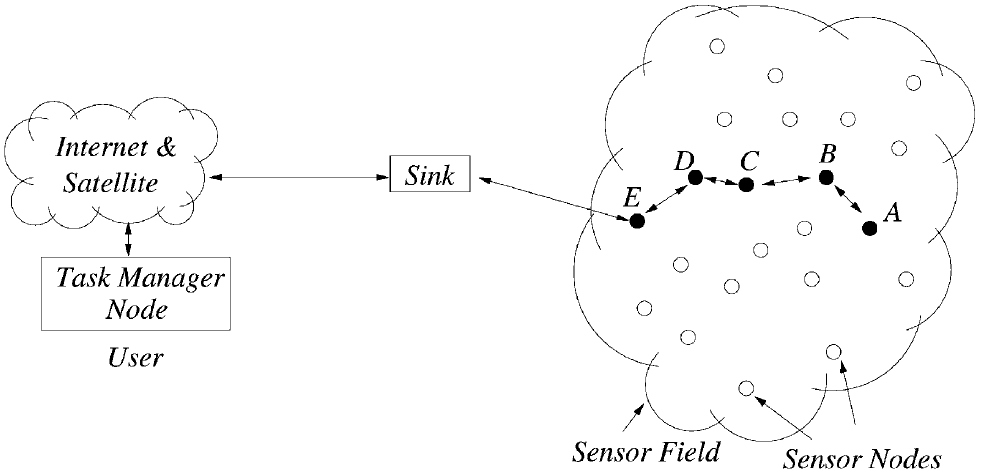
\includegraphics[scale=0.5]{Chapters/Figures/sensor_nodes_in_sensor_fields.png}
    \label{fig:sensor_nodes_in_sensor_fields}
\end{figure}

Typically, each node sensor is composed by a radio transceiver, an embedded processor, internal
and external memories, a power source and one or more sensors \cite{Wang2010}. However, the
nodes' design and the WSN itself' must take into account its purpose, the environment where
the nodes will operate, the hardware, the cost, along with other restrictions that need to
be considered \cite{Yick2008}.


\subsection{Architecture}
\label{subsec:wsn_architecture}
The most common architecture for WSN follows the OSI model. This model is composed of five
layers: application layer, transport layer, network layer, data link layer and physical layer,
and three cross plane layers: power management plane, mobility management plane and task
management plane, as shown in Fig. \ref{fig:wsn_architecture}.

\begin{figure}[h]
    \caption{WSN Architecture \cite{Akyildiz2002}}
    \centering
    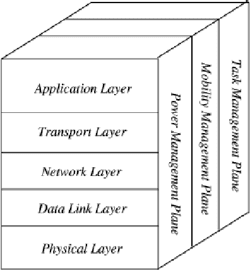
\includegraphics[scale=0.5]{Chapters/Figures/wsn_architecture.png}
    \label{fig:wsn_architecture}
\end{figure}

The five layers above mentioned work together to ensure the data is properly transmitted to the
network, each with a specific functionality:
% TODO: layers explanation
\begin{description}
    \item[Application Layer]
    \item[Transport Layer]
    \item[Network Layer]
    \item[Data Link Layer]
    \item[Physical Layer]
\end{description}

The management planes' roles are to manage the network and optimize the sensor nodes'
performance in order to improve the overall effectiveness of the network, considering the
advantages acquired by all sensor nodes working together. Each of these planes manages
a specific area \cite{Akyildiz2002}:
\begin{description}
    \item[Power Management Plane] manages how the sensor node uses its power, choosing when to
        turn off its receiver to save energy or to keep it from receiving repeated messages. It
        also informs its neighbours when it reaches a low power mode.
    \item[Mobility Management Plane:] keeps track of the sensor nodes' neighbours and always
        distinguishes a route back to the user.
    \item[Task Management Plane:] administers the periodicity and schedule that each node needs
        to maintain in order to perform their sensing tasks based on their power dependency and
        task requirements.
\end{description}

\subsection{Network Topologies}
There are several different topologies regarding the connection between nodes and their message
exchange routes \cite{Yadav2012, Lewis2004}:
\begin{description}
    \item[Star Topology:] all nodes are connected to only one node, the coordinator. This
        means every node will communicate via this central node and every node that requests
        to enter this network will have to send its information to the coordinator, which
        will then send it to the other nodes. The principal limitation of this topology is
        that if the coordinator malfunctions the whole network will fail.
    \item[Ring Topology:] all nodes are equal connected, having no coordinator. Contrarily
        to the star topology, if a single link is broken the whole network will fail.
    \item[Bus Topology:] all nodes broadcast their messages using the bus. Each message
        has a header with the destination address so that every node can see if the message
        is for them or another node. This topology is passive, since the nodes are not
        responsible for retransmitting messages.
    \item[Tree Topology:] similar to the star topology where the coordinator is the tree root, on
        the other hand the nodes at different levels of hierarchy are connected to sub-coordinators
        that lead to the root \cite{Shrestha2007}. In this topology, as in the star topology, if
        the coordinator malfunctions, the whole network will fail. However, differently from
        the star topology, will also have problems if a sub-coordinator fails as it will lead
        to the failure of every subordinate node.
    \item[Fully Connected Topology:] every node is connected to every other node. This will
        lead to a routing problem when dealing with large networks.
    \item[Mesh Topology:] the nodes are generally identical, so the mesh connections are
        commonly referred as peer-to-peer connections. However, even though the nodes are
        generally identical some of them can be assign as coordinators that take additional
        functions and if one of these coordinators stops working, another just takes over his
        work. An interesting aspect of this topology is that the communication can be
        done between any two nodes in close proximity, which makes this topology quite
        robust to the failure of nodes or links and good for large scale networks.
\end{description}

\begin{figure}[h]
    \caption{Network Topologies \cite{Lewis2004}}
    \centering
    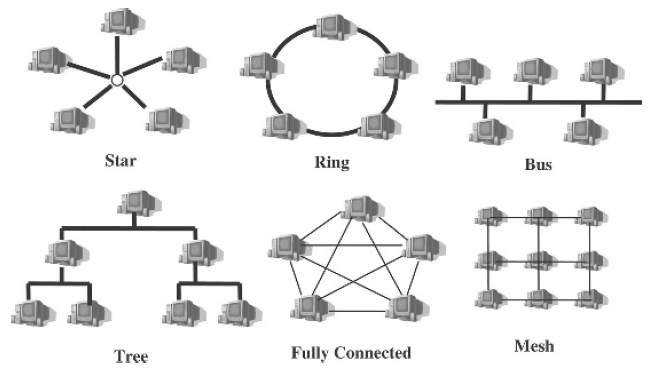
\includegraphics[scale=0.7]{Chapters/Figures/network_topologies.png}
    \label{fig:network_topologies}
\end{figure}

\subsection{Strategies}
\label{subsec:wsn_strategies}
% TODO:
The WSN have innumerous applications, this idea will be further discussed in the subsequent
subsection \ref{subsec:wsn_applications}, which will lead to different solutions for each of
them.

\subsection{Gossip in WSNs}
\label{subsec:gossip_in_wsns}
One of the main purposes of a sensor node is to transmit the data it has collected, via
the sensors, to the sink. The route chosen by these nodes is of the most importance,
therefore various protocols were studied in \cite{Akkaya2005} to understand which of
these would better conduct this task.

As presented previously in the section \ref{sec:gossip_protocol}, during the gossip protocol
each node only transmits its messages to \textit{t} randomly selected nodes and not the
whole network, as in the flooding protocol. This characteristic ensures that every node
in the gossip protocol will only have a single copy of the packet to be sent, which
addresses one of the shortcomings of the flooding protocol, the implosion. However, this
will lead to delays in the dissemination of the data which may be an important factor
for some applications of the network.

\subsection{Applications}
\label{subsec:wsn_applications}
Due to the fact that the sensor nodes in a WSN may collect distinct types of data, based on
sensing task and the sensor itself, there are many applications and subsequentially many are
areas of expertise in WSR. These areas may be related to health, the military, home,
environmental, commercial and many more. For this thesis it is more impactful to learn about
some of the applications in the tracking area, per example, \nameref{subsubsection:zebranet}
and \nameref{subsubsection:wireless_tracking}.

\subsubsection{ZebraNet}
\label{subsubsection:zebranet}
One of the most revolutionary applications of WSN is the ZebraNet, a method developed to
track wildlife specifically, zebras, for biology research, using a mobile base station. The
ZebraNet collects logged data from tracking collars, transported by the
animals, and afterward it transmits this data back to the researchers. Considering there
is no fixed antennas or cellular telephone service, the protocol uses ad hoc
peer-to-peer routing to transport the data around.

The ZebraNet project focused on resolving some of the problems observed from previous
studies of collecting data from wildlife tracking. One of the main obstacles was using
satellites to transport the data. The process of uploading data to satellites is slow and
power consuming. Moreover, the data download from the satellite to the researchers is
charged by the bit, which restricted the amount of data collected. Furthermore, these
systems used batteries without solar recharge, which would eventually end, and had to be
recovered and recharged, losing enormous amounts of data in process \cite{Juang2002}.

Additional, one of the biggest concerns during the development of this project was the
design limitations. Due to the fact that each node would be transported by an animal,
its weight and size was immediately limited. And since the nodes are difficult to
retrieve, the device has to have a durable battery life \cite{Zhang2004}. Subsequentially,
most of the weight would be occupied by the battery and the GPS, leaving a small
space for the storage, which means that there is small space for redundant messages in this
protocol. Lastly, it was crucial to consider the impact of the number and size of data
transmissions required as well as the range of these transmissions.
% TODO: maybe talk more about the hardware
% TODO: conclude

\subsubsection{Wireless Tracking}
\label{subsubsection:wireless_tracking}
Wireless tracking is an application widely common when dealing with wildlife research. Usually,
it takes the sensor direct position with the use of GPS to track the node itself. There is,
however, another method to obtain this position. It can be estimated using the information
from the surrounding nodes. This method is called remote positioning and it is truly relevant
when it is necessary to reduce resources consumption. To have a functional wireless tracking
it is, nonetheless, vital to have an accurate position.



\subsection{WSN Challenges}
% Challenges of WSN: 
% Quality of Service
% Security Issue
% Energy Efficiency
% Network Throughput
% Performance
% Ability to cope with node failure
% Cross layer optimisation
% Scalability to large scale of deployment

\subsection{Discussion}
%discussion -> most important is the low power
% -> zebranet has mobile base station, zebra-tracking is a domain in which the
% node mobility models are largely unknown, and in fact are ultimately the research goal.
% -> https://books.google.pt/books?hl=pt-PT&lr=&id=4zyDBwAAQBAJ&oi=fnd&pg=PA21&dq=wireless+sensor+networks&ots=6jAD4wkz4u&sig=f31E5q7e1haSQHXUagmjlYs3LnE&redir_esc=y#v=onepage&q&f=false
% 1.5.3 Automatic Localization and Time Synchronization


%\section{Sensors and Arduino}
%\label{sec:sensors_and_arduino}

\section{Existing Collars}
\label{sec:existing_collars}


\section{Cows}
\label{sec:cows}
Some animals are known to form subgroups to perform their everyday tasks. In the case of
cows, these groups are called herds and they distinguish three main activities: resting,
grazing and travelling. We will discuss next how cows behave.

\subsection{Cattle Behaviour in Herds}
\label{subsec:behaviour_herds}
The cows follow a hierarchical system, where the oldest cow is regularly the leader of the
herd. Scarcely, there is a younger, stronger, cow leading a group \cite{Harris2007}. This
leader can choose where the herd moves, having influence over the other cows that follow her.
This effect is more pronounced when the herd is travelling in comparison to when they are
grazing or resting \cite{Vsarova2010}.

There was conducted a study that observed the interactions of cows during the course of two
years. During this research it was reached some interesting conclusion about the proximity
demonstrated by these animals. It was found a correlation between the distance of neighbours
in a herd and the quantity of pasturage available. When there is abundant nourishment, the
herd are more compact, and the animals graze closer together \cite{Harris2007}.

\subsection{Diet Impact on Plant Communities}
\label{subsec:diet}
The diet of an animal has a profound impact on the quality of the products derived from it \cite{Araujo2014}.
Therefore, it is reasonably for farm owners to feed their cattle with natural vegetation, when
possible, instead of synthetic one.

In 2018, it was conducted a study in the Netherlands that distinguished the dieting habits of
three species: cattle, bison and horses \cite{Cromsigt2018}. During this study it was
discovered that the cattle eating habits, in a landscape without supplementary feeding,
consisted mostly on grass (around 80\%) and woody plants, twigs and leaves, (around 20\%). It
was supposed that the consume of woody plants was derived from the lack of grass during the
winter. Without the data from a similar study convened in Portugal, we can only presume that
with the more favorable climatic conditions the cattle would feed almost completely on grass.

A study was convened on three ranches in Texas with the purpose of understanding the impact
of distinct types of grazing on the soil and vegetation. In the first ranch it was used the
multi-paddock technique, in the second one it was used light continuous grazing and in the
last one it was used heavy continuous grazing. With the multi-paddock method, the terrain is
divided in multiple smaller paddocks and regularly each herd rotates from one paddock to the
next. In the end, it was concluded that this type of grazing management is overall better for
the soil and vegetation that the light or the heavy continuous grazing methods \cite{Teague2011}

\subsection{Discussion}
\label{subsec:cow_discussion}
It is imperative to understand how cows operate to correctly develop a tracking system that
works for them and considers their behaviour.

Comprehending the relation and the distance between individual cows and their neighbours is
of utmost importance for my future work, considering that the messages collected from each
cow will have to be disseminated using a peer-to-peer based protocol.

Furthermore, it is fundamental to consider in my next steps that the farm owners should be able
to shift the grazing location of the herds to obtain a wealthier vegetation and soil, leading
to overall better cattle.


\section{Summary}
\label{sec:summary}
% ad hoc protocol -> An ad hoc protocol is a type of communication protocol that allows 
% devices to connect and communicate with each other without the need for a central 
% network infrastructure or access point. In an ad hoc network, each device acts as a 
% router, forwarding packets to other devices on the network. This type of network is 
% often used in situations where a traditional network infrastructure is not available or 
% feasible, such as in emergency or disaster scenarios, or in mobile or wireless 
% environments.